
The fundamental innovation in this research is the integrative combination of transcranial super-resolution ultrasound imaging with targeted sonothrombolysis in a single, co-registered platform for stroke diagnosis and treatment. No existing system combines micron-resolution neurovascular imaging with precision-focused therapeutic ultrasound delivery through the intact skull. Innovative aspects introduced in this proposal include:

\subsection{Non-invasive volumetric whole-brain transcranial imaging:} The skull is a barrier for ultrasound. Imaging tools developed here overcome these challenges through innovation in dual-frequency imaging, where the low frequency more easily penetrates the skull, phase aberration correction which reduces focal degradation, large-aperture sparse arrays which maintain small F-numbers at depth, and contrast agents which improve signal brightness. Although there is no silver bullet for transcranial ultrasound imaging, combining innovation on several fronts will generate high-contrast high-resolution (up to 10~$\mu$m) non-invasive transcranial images of the whole \textit{in vivo} brain.

\subsection{Innovation in super-harmonic super-resolution imaging:} Conventional super-resolution imaging relies on spatiotemporal filtering, which cannot image stationary or slow-moving targets such as microbubbles lodged at or near a thrombus. Our innovation of super-harmonic super-resolution overcomes this barrier by relying on dual-frequency imaging to separate contrast agent signal from tissue signal based on nonlinear resonance physics, enabling super-resolved localization of both freely circulating and stationary microbubbles~\cite{kierski2020super,kierski2020superharmonic,kierski2022acoustic}.

\begin{wrapfigure}{r}{0.46\textwidth}
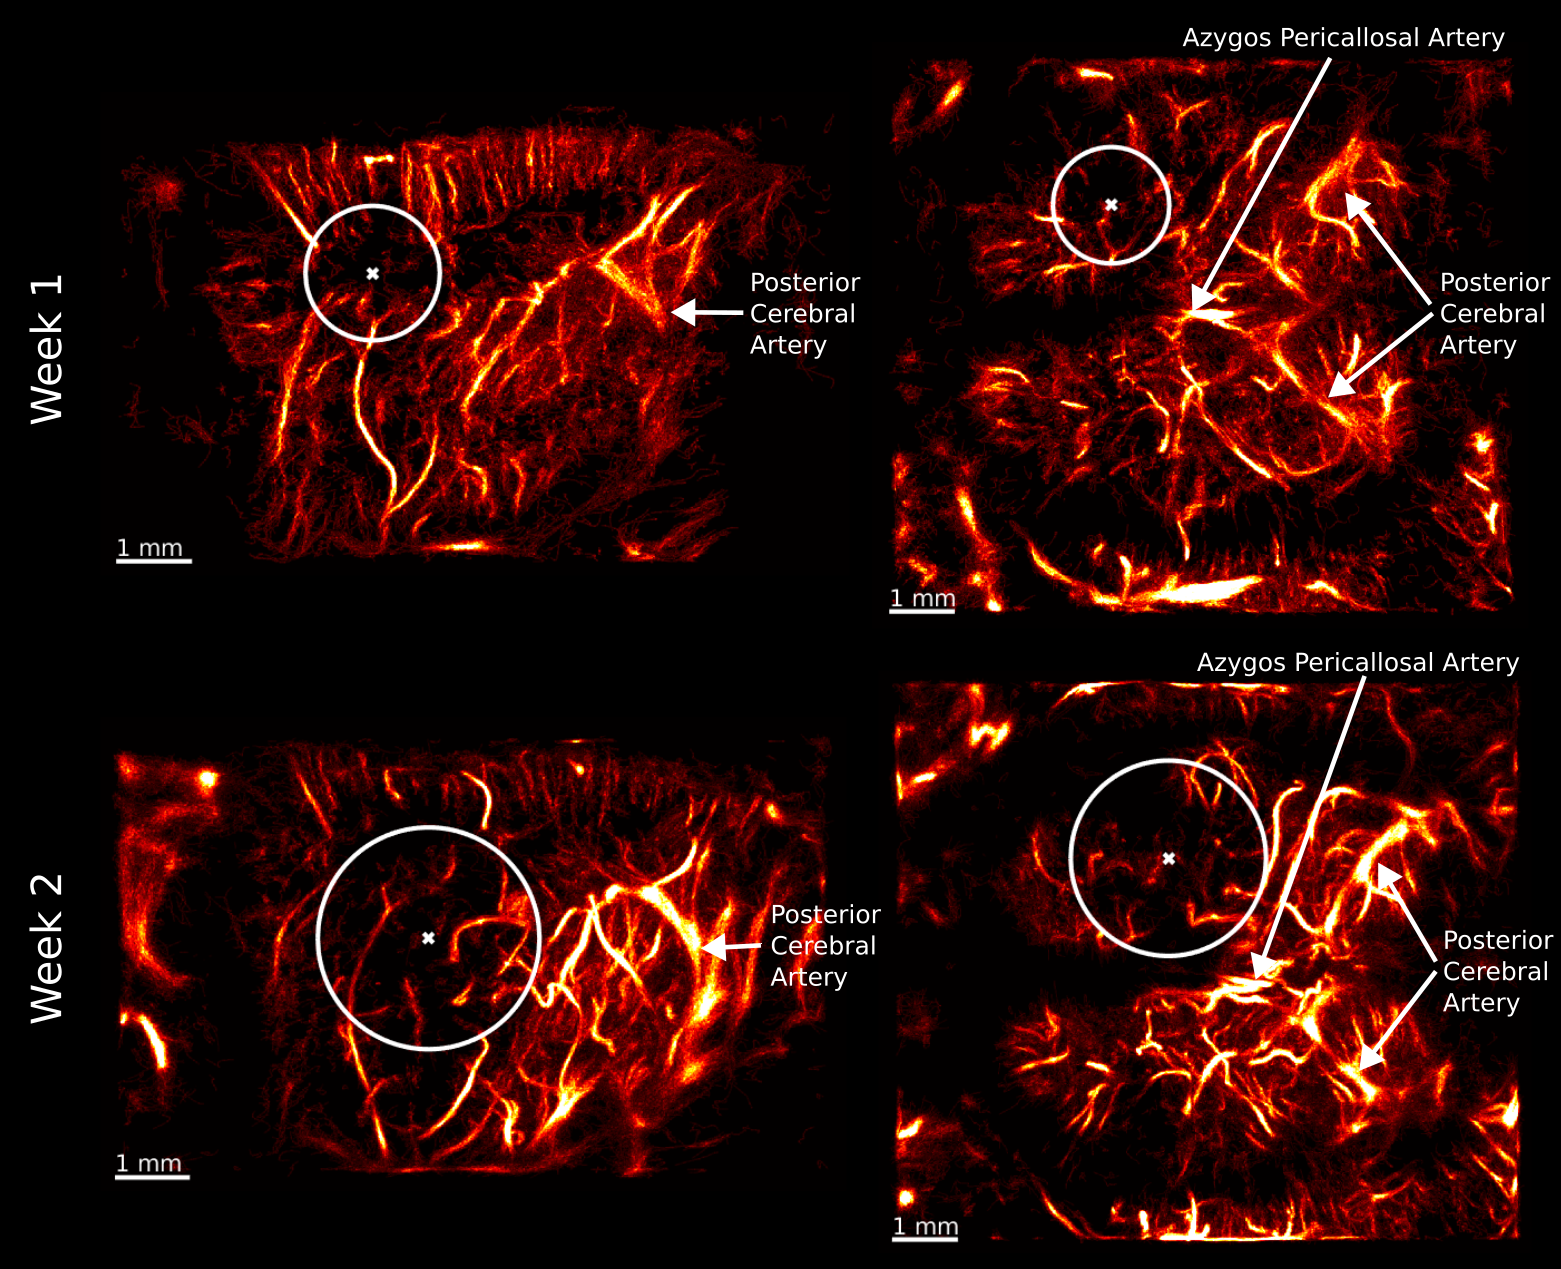
\includegraphics[width=0.46\textwidth]{figures/ULM_I_m977_LabeledVessels.png}
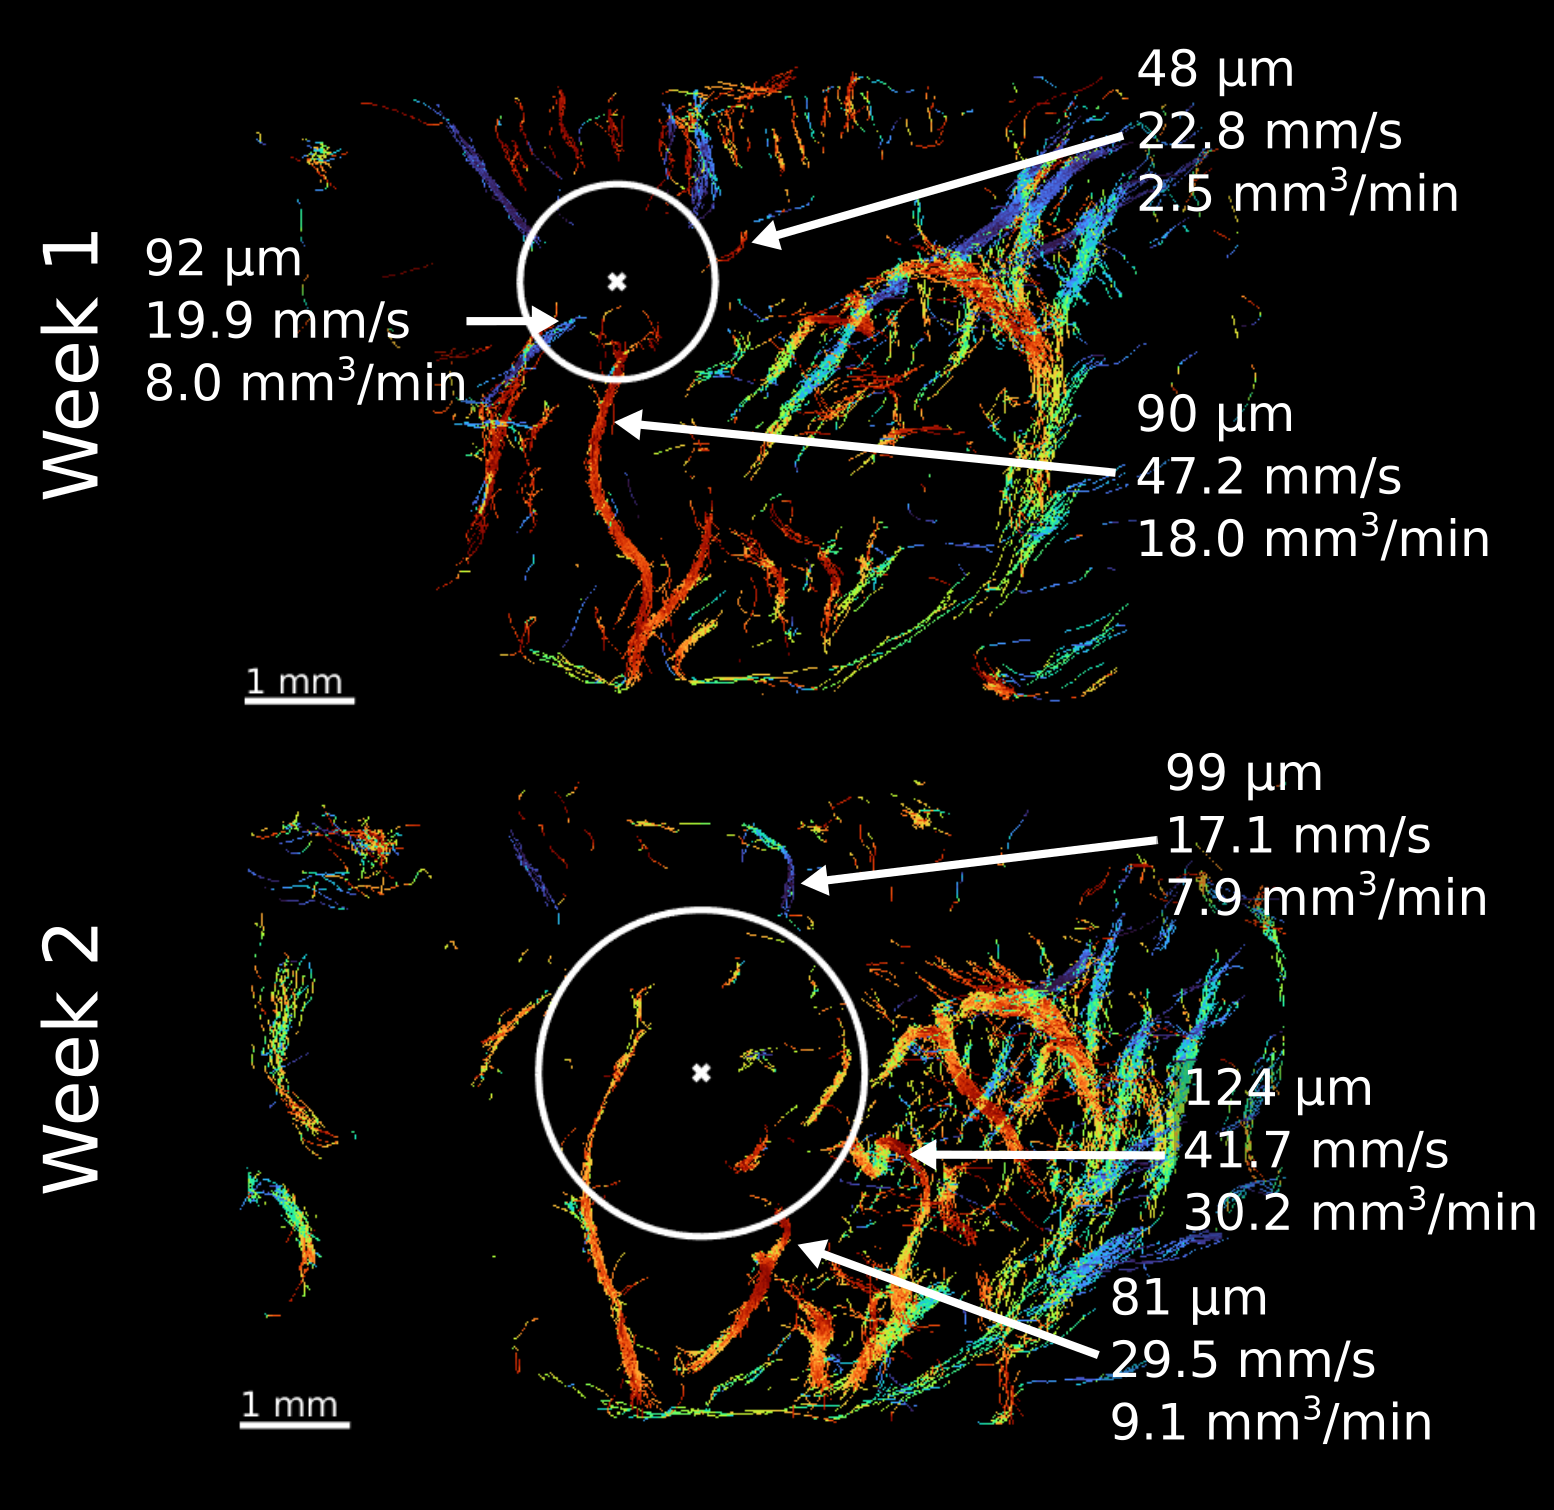
\includegraphics[width=0.25\textwidth]{figures/ULM_Proj_m977_LabeledMetrics.png}
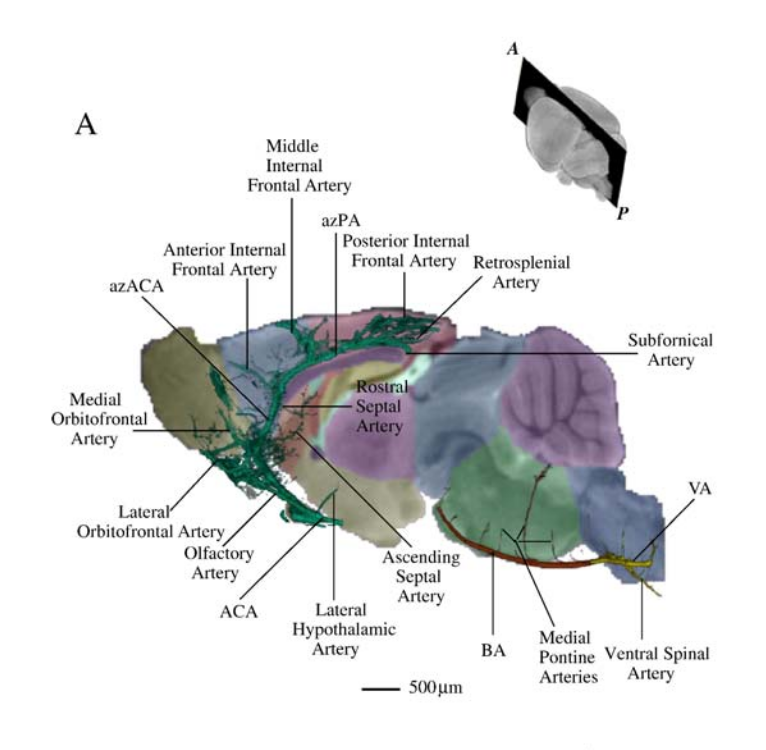
\includegraphics[width=0.2\textwidth]{figures/Screenshot from 2023-09-29 17-17-51.png}
\caption{\label{fig:gbm_quantification} Non-invasive whole-brain volumetric super-resolution images for sagittal and coronal views of a rodent brain at week 1 and 2 (top). Quantitative microvascular characterization of vessel diameter, blood speed, and flow (bottom left). Identification of individual vessels via atlas co-registration (bottom right).}
\vspace{-0.5cm}
\end{wrapfigure}

\subsection{Dual-frequency array design:} Low frequencies penetrate the skull more effectively, making them ideal for both high-power therapeutic delivery and for super-harmonic imaging which relies on broad bandwidth separation. Our dual-frequency array design combines these functions into a single device that delivers both low-frequency super-harmonic imaging transmits and focused sonothrombolytic pulses, while a co-integrated receive array captures the broadband microbubble response.

\subsection{Co-registration of imaging and therapy:} Since the imaging and therapeutic beams share the same acoustic path through the skull, they are physically co-registered and robust to residual skull aberration. Aberration correction applied for imaging simultaneously corrects the therapeutic focus. The thrombus localized by super-resolution imaging is, by construction, the target for sonothrombolysis---no registration error, no coordinate transformation, and no susceptibility to brain shift.

\subsection{Precision targeted sonothrombolysis with real-time feedback:} Prior sonothrombolysis approaches insonified hundreds of cm$^3$ of brain with unfocused beams. Our approach confines the therapeutic focal volume to a few~mm$^3$ at the clot (750~$\mu$m diameter, 50~$\mu$m positional accuracy), delivering orders-of-magnitude higher energy density at the thrombus while sparing surrounding tissue. Concurrent super-resolution imaging provides real-time microvascular-level feedback on reperfusion, enabling a closed-loop paradigm: localize, treat, monitor, adjust.

\subsection{Microbubbles as integrated theranostic agents:} A single microbubble population serves both diagnostic and therapeutic functions---providing the point sources for super-resolution localization and the cavitation nuclei for sonothrombolysis. Microbubbles circulating through partially recanalized vessels simultaneously provide imaging feedback on reperfusion while enhancing ongoing thrombolysis, coupling the diagnostic and therapeutic functions through the same physical medium.
